% Created by tikzDevice version 0.6.2-92-0ad2792 on 2013-01-08 03:49:56
% !TEX encoding = UTF-8 Unicode
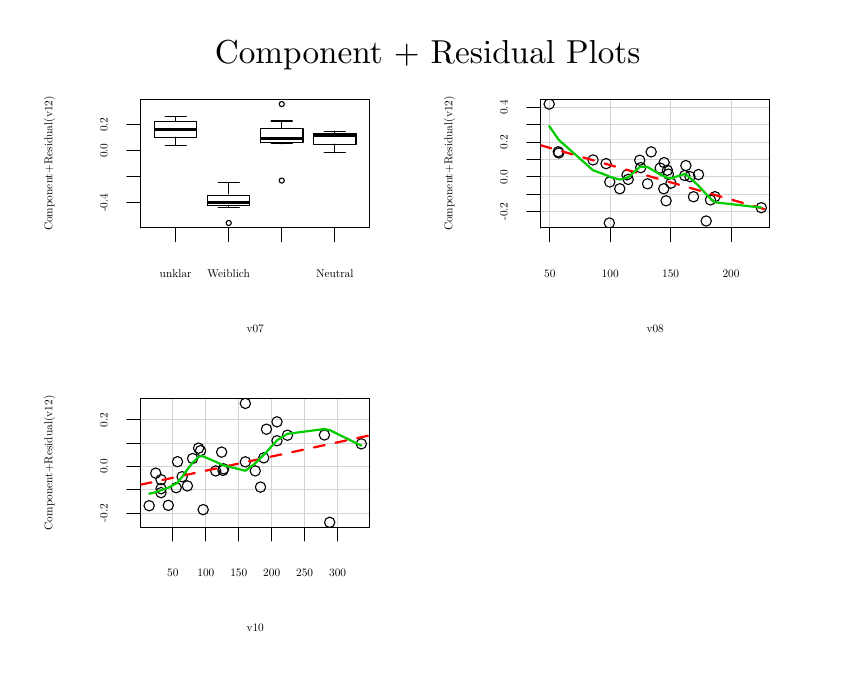
\begin{tikzpicture}[x=1pt,y=1pt]
\definecolor[named]{fillColor}{rgb}{1.00,1.00,1.00}
\path[use as bounding box,fill=fillColor,fill opacity=0.00] (0,0) rectangle (289.08,231.26);
\begin{scope}
\path[clip] ( 40.84,158.96) rectangle (123.62,205.37);
\definecolor[named]{drawColor}{rgb}{0.00,0.00,0.00}

\path[draw=drawColor,line width= 1.2pt,line join=round] ( 45.82,194.42) -- ( 61.15,194.42);

\path[draw=drawColor,line width= 0.4pt,dash pattern=on 4pt off 4pt ,line join=round,line cap=round] ( 53.48,188.66) -- ( 53.48,191.69);

\path[draw=drawColor,line width= 0.4pt,dash pattern=on 4pt off 4pt ,line join=round,line cap=round] ( 53.48,199.20) -- ( 53.48,197.37);

\path[draw=drawColor,line width= 0.4pt,line join=round,line cap=round] ( 49.65,188.66) -- ( 57.32,188.66);

\path[draw=drawColor,line width= 0.4pt,line join=round,line cap=round] ( 49.65,199.20) -- ( 57.32,199.20);

\path[draw=drawColor,line width= 0.4pt,line join=round,line cap=round] ( 45.82,191.69) --
	( 61.15,191.69) --
	( 61.15,197.37) --
	( 45.82,197.37) --
	( 45.82,191.69);

\path[draw=drawColor,line width= 1.2pt,line join=round] ( 64.98,168.02) -- ( 80.31,168.02);

\path[draw=drawColor,line width= 0.4pt,dash pattern=on 4pt off 4pt ,line join=round,line cap=round] ( 72.65,166.23) -- ( 72.65,167.09);

\path[draw=drawColor,line width= 0.4pt,dash pattern=on 4pt off 4pt ,line join=round,line cap=round] ( 72.65,175.18) -- ( 72.65,170.46);

\path[draw=drawColor,line width= 0.4pt,line join=round,line cap=round] ( 68.82,166.23) -- ( 76.48,166.23);

\path[draw=drawColor,line width= 0.4pt,line join=round,line cap=round] ( 68.82,175.18) -- ( 76.48,175.18);

\path[draw=drawColor,line width= 0.4pt,line join=round,line cap=round] ( 64.98,167.09) --
	( 80.31,167.09) --
	( 80.31,170.46) --
	( 64.98,170.46) --
	( 64.98,167.09);

\path[draw=drawColor,line width= 0.4pt,line join=round,line cap=round] ( 72.65,160.68) circle (  0.93);

\path[draw=drawColor,line width= 1.2pt,line join=round] ( 84.15,191.11) -- ( 99.48,191.11);

\path[draw=drawColor,line width= 0.4pt,dash pattern=on 4pt off 4pt ,line join=round,line cap=round] ( 91.81,189.31) -- ( 91.81,189.65);

\path[draw=drawColor,line width= 0.4pt,dash pattern=on 4pt off 4pt ,line join=round,line cap=round] ( 91.81,197.53) -- ( 91.81,194.86);

\path[draw=drawColor,line width= 0.4pt,line join=round,line cap=round] ( 87.98,189.31) -- ( 95.64,189.31);

\path[draw=drawColor,line width= 0.4pt,line join=round,line cap=round] ( 87.98,197.53) -- ( 95.64,197.53);

\path[draw=drawColor,line width= 0.4pt,line join=round,line cap=round] ( 84.15,189.65) --
	( 99.48,189.65) --
	( 99.48,194.86) --
	( 84.15,194.86) --
	( 84.15,189.65);

\path[draw=drawColor,line width= 0.4pt,line join=round,line cap=round] ( 91.81,176.00) circle (  0.93);

\path[draw=drawColor,line width= 0.4pt,line join=round,line cap=round] ( 91.81,203.65) circle (  0.93);

\path[draw=drawColor,line width= 1.2pt,line join=round] (103.31,192.34) -- (118.64,192.34);

\path[draw=drawColor,line width= 0.4pt,dash pattern=on 4pt off 4pt ,line join=round,line cap=round] (110.98,186.05) -- (110.98,189.19);

\path[draw=drawColor,line width= 0.4pt,dash pattern=on 4pt off 4pt ,line join=round,line cap=round] (110.98,193.61) -- (110.98,192.97);

\path[draw=drawColor,line width= 0.4pt,line join=round,line cap=round] (107.14,186.05) -- (114.81,186.05);

\path[draw=drawColor,line width= 0.4pt,line join=round,line cap=round] (107.14,193.61) -- (114.81,193.61);

\path[draw=drawColor,line width= 0.4pt,line join=round,line cap=round] (103.31,189.19) --
	(118.64,189.19) --
	(118.64,192.97) --
	(103.31,192.97) --
	(103.31,189.19);
\end{scope}
\begin{scope}
\path[clip] (  0.00,  0.00) rectangle (289.08,231.26);
\definecolor[named]{drawColor}{rgb}{0.00,0.00,0.00}

\path[draw=drawColor,line width= 0.4pt,line join=round,line cap=round] ( 53.48,158.96) -- (110.98,158.96);

\path[draw=drawColor,line width= 0.4pt,line join=round,line cap=round] ( 53.48,158.96) -- ( 53.48,153.98);

\path[draw=drawColor,line width= 0.4pt,line join=round,line cap=round] ( 72.65,158.96) -- ( 72.65,153.98);

\path[draw=drawColor,line width= 0.4pt,line join=round,line cap=round] ( 91.81,158.96) -- ( 91.81,153.98);

\path[draw=drawColor,line width= 0.4pt,line join=round,line cap=round] (110.98,158.96) -- (110.98,153.98);

\node[text=drawColor,anchor=base,inner sep=0pt, outer sep=0pt, scale=  0.41] at ( 53.48,141.03) {unklar};

\node[text=drawColor,anchor=base,inner sep=0pt, outer sep=0pt, scale=  0.41] at ( 72.65,141.03) {Weiblich};

\node[text=drawColor,anchor=base,inner sep=0pt, outer sep=0pt, scale=  0.41] at (110.98,141.03) {Neutral};

\path[draw=drawColor,line width= 0.4pt,line join=round,line cap=round] ( 40.84,168.00) -- ( 40.84,196.24);

\path[draw=drawColor,line width= 0.4pt,line join=round,line cap=round] ( 40.84,168.00) -- ( 35.86,168.00);

\path[draw=drawColor,line width= 0.4pt,line join=round,line cap=round] ( 40.84,177.41) -- ( 35.86,177.41);

\path[draw=drawColor,line width= 0.4pt,line join=round,line cap=round] ( 40.84,186.82) -- ( 35.86,186.82);

\path[draw=drawColor,line width= 0.4pt,line join=round,line cap=round] ( 40.84,196.24) -- ( 35.86,196.24);

\node[text=drawColor,rotate= 90.00,anchor=base,inner sep=0pt, outer sep=0pt, scale=  0.41] at ( 28.88,168.00) {-0.4};

\node[text=drawColor,rotate= 90.00,anchor=base,inner sep=0pt, outer sep=0pt, scale=  0.41] at ( 28.88,186.82) {0.0};

\node[text=drawColor,rotate= 90.00,anchor=base,inner sep=0pt, outer sep=0pt, scale=  0.41] at ( 28.88,196.24) {0.2};
\end{scope}
\begin{scope}
\path[clip] (  0.00,108.16) rectangle (144.54,216.32);
\definecolor[named]{drawColor}{rgb}{0.00,0.00,0.00}

\node[text=drawColor,anchor=base,inner sep=0pt, outer sep=0pt, scale=  0.41] at ( 82.23,121.11) {v07};

\node[text=drawColor,rotate= 90.00,anchor=base,inner sep=0pt, outer sep=0pt, scale=  0.41] at (  8.96,182.16) {Component+Residual(v12)};
\end{scope}
\begin{scope}
\path[clip] (  0.00,  0.00) rectangle (289.08,231.26);
\definecolor[named]{drawColor}{rgb}{0.00,0.00,0.00}

\path[draw=drawColor,line width= 0.4pt,line join=round,line cap=round] ( 40.84,158.96) --
	(123.62,158.96) --
	(123.62,205.37) --
	( 40.84,205.37) --
	( 40.84,158.96);
\end{scope}
\begin{scope}
\path[clip] (  0.00,  0.00) rectangle (289.08,231.26);
\definecolor[named]{drawColor}{rgb}{0.00,0.00,0.00}

\path[draw=drawColor,line width= 0.4pt,line join=round,line cap=round] (188.66,158.96) -- (254.17,158.96);

\path[draw=drawColor,line width= 0.4pt,line join=round,line cap=round] (188.66,158.96) -- (188.66,153.98);

\path[draw=drawColor,line width= 0.4pt,line join=round,line cap=round] (210.50,158.96) -- (210.50,153.98);

\path[draw=drawColor,line width= 0.4pt,line join=round,line cap=round] (232.34,158.96) -- (232.34,153.98);

\path[draw=drawColor,line width= 0.4pt,line join=round,line cap=round] (254.17,158.96) -- (254.17,153.98);

\node[text=drawColor,anchor=base,inner sep=0pt, outer sep=0pt, scale=  0.41] at (188.66,141.03) {50};

\node[text=drawColor,anchor=base,inner sep=0pt, outer sep=0pt, scale=  0.41] at (210.50,141.03) {100};

\node[text=drawColor,anchor=base,inner sep=0pt, outer sep=0pt, scale=  0.41] at (232.34,141.03) {150};

\node[text=drawColor,anchor=base,inner sep=0pt, outer sep=0pt, scale=  0.41] at (254.17,141.03) {200};

\path[draw=drawColor,line width= 0.4pt,line join=round,line cap=round] (185.38,164.82) -- (185.38,202.39);

\path[draw=drawColor,line width= 0.4pt,line join=round,line cap=round] (185.38,164.82) -- (180.40,164.82);

\path[draw=drawColor,line width= 0.4pt,line join=round,line cap=round] (185.38,171.08) -- (180.40,171.08);

\path[draw=drawColor,line width= 0.4pt,line join=round,line cap=round] (185.38,177.34) -- (180.40,177.34);

\path[draw=drawColor,line width= 0.4pt,line join=round,line cap=round] (185.38,183.60) -- (180.40,183.60);

\path[draw=drawColor,line width= 0.4pt,line join=round,line cap=round] (185.38,189.86) -- (180.40,189.86);

\path[draw=drawColor,line width= 0.4pt,line join=round,line cap=round] (185.38,196.12) -- (180.40,196.12);

\path[draw=drawColor,line width= 0.4pt,line join=round,line cap=round] (185.38,202.39) -- (180.40,202.39);

\node[text=drawColor,rotate= 90.00,anchor=base,inner sep=0pt, outer sep=0pt, scale=  0.41] at (173.42,164.82) {-0.2};

\node[text=drawColor,rotate= 90.00,anchor=base,inner sep=0pt, outer sep=0pt, scale=  0.41] at (173.42,177.34) {0.0};

\node[text=drawColor,rotate= 90.00,anchor=base,inner sep=0pt, outer sep=0pt, scale=  0.41] at (173.42,189.86) {0.2};

\node[text=drawColor,rotate= 90.00,anchor=base,inner sep=0pt, outer sep=0pt, scale=  0.41] at (173.42,202.39) {0.4};

\path[draw=drawColor,line width= 0.4pt,line join=round,line cap=round] (185.38,158.96) --
	(268.16,158.96) --
	(268.16,205.37) --
	(185.38,205.37) --
	(185.38,158.96);
\end{scope}
\begin{scope}
\path[clip] (144.54,108.16) rectangle (289.08,216.32);
\definecolor[named]{drawColor}{rgb}{0.00,0.00,0.00}

\node[text=drawColor,anchor=base,inner sep=0pt, outer sep=0pt, scale=  0.41] at (226.77,121.11) {v08};

\node[text=drawColor,rotate= 90.00,anchor=base,inner sep=0pt, outer sep=0pt, scale=  0.41] at (153.50,182.16) {Component+Residual(v12)};
\end{scope}
\begin{scope}
\path[clip] (185.38,158.96) rectangle (268.16,205.37);
\definecolor[named]{drawColor}{rgb}{0.83,0.83,0.83}

\path[draw=drawColor,line width= 0.4pt,line join=round,line cap=round] (188.66,158.96) -- (188.66,205.37);

\path[draw=drawColor,line width= 0.4pt,line join=round,line cap=round] (210.50,158.96) -- (210.50,205.37);

\path[draw=drawColor,line width= 0.4pt,line join=round,line cap=round] (232.34,158.96) -- (232.34,205.37);

\path[draw=drawColor,line width= 0.4pt,line join=round,line cap=round] (254.17,158.96) -- (254.17,205.37);

\path[draw=drawColor,line width= 0.4pt,line join=round,line cap=round] (185.38,164.82) -- (268.16,164.82);

\path[draw=drawColor,line width= 0.4pt,line join=round,line cap=round] (185.38,171.08) -- (268.16,171.08);

\path[draw=drawColor,line width= 0.4pt,line join=round,line cap=round] (185.38,177.34) -- (268.16,177.34);

\path[draw=drawColor,line width= 0.4pt,line join=round,line cap=round] (185.38,183.60) -- (268.16,183.60);

\path[draw=drawColor,line width= 0.4pt,line join=round,line cap=round] (185.38,189.86) -- (268.16,189.86);

\path[draw=drawColor,line width= 0.4pt,line join=round,line cap=round] (185.38,196.12) -- (268.16,196.12);

\path[draw=drawColor,line width= 0.4pt,line join=round,line cap=round] (185.38,202.39) -- (268.16,202.39);
\end{scope}
\begin{scope}
\path[clip] (  0.00,  0.00) rectangle (289.08,231.26);
\definecolor[named]{drawColor}{rgb}{0.00,0.00,0.00}

\path[draw=drawColor,line width= 0.4pt,line join=round,line cap=round] (185.38,158.96) --
	(268.16,158.96) --
	(268.16,205.37) --
	(185.38,205.37) --
	(185.38,158.96);
\end{scope}
\begin{scope}
\path[clip] (185.38,158.96) rectangle (268.16,205.37);
\definecolor[named]{drawColor}{rgb}{0.00,0.00,0.00}

\path[draw=drawColor,line width= 0.4pt,line join=round,line cap=round] (231.16,179.72) circle (  1.87);

\path[draw=drawColor,line width= 0.4pt,line join=round,line cap=round] (230.69,168.70) circle (  1.87);

\path[draw=drawColor,line width= 0.4pt,line join=round,line cap=round] (239.31,177.42) circle (  1.87);

\path[draw=drawColor,line width= 0.4pt,line join=round,line cap=round] (213.95,173.05) circle (  1.87);

\path[draw=drawColor,line width= 0.4pt,line join=round,line cap=round] (204.28,183.46) circle (  1.87);

\path[draw=drawColor,line width= 0.4pt,line join=round,line cap=round] (209.00,182.12) circle (  1.87);

\path[draw=drawColor,line width= 0.4pt,line join=round,line cap=round] (229.98,182.50) circle (  1.87);

\path[draw=drawColor,line width= 0.4pt,line join=round,line cap=round] (245.18,161.40) circle (  1.87);

\path[draw=drawColor,line width= 0.4pt,line join=round,line cap=round] (242.40,178.17) circle (  1.87);

\path[draw=drawColor,line width= 0.4pt,line join=round,line cap=round] (248.32,170.18) circle (  1.87);

\path[draw=drawColor,line width= 0.4pt,line join=round,line cap=round] (225.29,186.37) circle (  1.87);

\path[draw=drawColor,line width= 0.4pt,line join=round,line cap=round] (232.44,175.08) circle (  1.87);

\path[draw=drawColor,line width= 0.4pt,line join=round,line cap=round] (223.99,174.84) circle (  1.87);

\path[draw=drawColor,line width= 0.4pt,line join=round,line cap=round] (191.72,186.41) circle (  1.87);

\path[draw=drawColor,line width= 0.4pt,line join=round,line cap=round] (265.10,166.20) circle (  1.87);

\path[draw=drawColor,line width= 0.4pt,line join=round,line cap=round] (246.72,169.02) circle (  1.87);

\path[draw=drawColor,line width= 0.4pt,line join=round,line cap=round] (217.01,176.43) circle (  1.87);

\path[draw=drawColor,line width= 0.4pt,line join=round,line cap=round] (228.54,180.52) circle (  1.87);

\path[draw=drawColor,line width= 0.4pt,line join=round,line cap=round] (231.52,178.33) circle (  1.87);

\path[draw=drawColor,line width= 0.4pt,line join=round,line cap=round] (210.17,160.68) circle (  1.87);

\path[draw=drawColor,line width= 0.4pt,line join=round,line cap=round] (237.84,181.43) circle (  1.87);

\path[draw=drawColor,line width= 0.4pt,line join=round,line cap=round] (229.85,173.05) circle (  1.87);

\path[draw=drawColor,line width= 0.4pt,line join=round,line cap=round] (188.44,203.65) circle (  1.87);

\path[draw=drawColor,line width= 0.4pt,line join=round,line cap=round] (240.59,170.16) circle (  1.87);

\path[draw=drawColor,line width= 0.4pt,line join=round,line cap=round] (216.58,178.08) circle (  1.87);

\path[draw=drawColor,line width= 0.4pt,line join=round,line cap=round] (191.92,185.97) circle (  1.87);

\path[draw=drawColor,line width= 0.4pt,line join=round,line cap=round] (221.16,183.36) circle (  1.87);

\path[draw=drawColor,line width= 0.4pt,line join=round,line cap=round] (221.52,180.68) circle (  1.87);

\path[draw=drawColor,line width= 0.4pt,line join=round,line cap=round] (210.34,175.50) circle (  1.87);

\path[draw=drawColor,line width= 0.4pt,line join=round,line cap=round] (237.41,177.84) circle (  1.87);
\definecolor[named]{drawColor}{rgb}{1.00,0.00,0.00}

\path[draw=drawColor,line width= 0.8pt,dash pattern=on 4pt off 4pt ,line join=round,line cap=round] (185.38,188.76) -- (268.16,165.16);
\definecolor[named]{drawColor}{rgb}{0.00,0.80,0.00}

\path[draw=drawColor,line width= 0.8pt,line join=round,line cap=round] (188.44,195.73) --
	(191.72,190.98) --
	(191.92,190.71) --
	(204.28,179.74) --
	(209.00,178.00) --
	(210.17,177.48) --
	(210.34,177.39) --
	(213.95,176.35) --
	(216.58,177.03) --
	(217.01,177.19) --
	(221.16,180.90) --
	(221.52,181.08) --
	(223.99,180.87) --
	(225.29,180.14) --
	(228.54,178.19) --
	(229.85,177.61) --
	(229.98,177.56) --
	(230.69,177.20) --
	(231.16,176.98) --
	(231.52,176.91) --
	(232.44,176.84) --
	(237.41,178.37) --
	(237.84,178.20) --
	(239.31,177.01) --
	(240.59,175.82) --
	(242.40,174.14) --
	(245.18,171.11) --
	(246.72,169.53) --
	(248.32,168.16) --
	(265.10,166.24);
\end{scope}
\begin{scope}
\path[clip] (  0.00,  0.00) rectangle (289.08,231.26);
\definecolor[named]{drawColor}{rgb}{0.00,0.00,0.00}

\path[draw=drawColor,line width= 0.4pt,line join=round,line cap=round] ( 52.47, 50.80) -- (111.99, 50.80);

\path[draw=drawColor,line width= 0.4pt,line join=round,line cap=round] ( 52.47, 50.80) -- ( 52.47, 45.82);

\path[draw=drawColor,line width= 0.4pt,line join=round,line cap=round] ( 64.38, 50.80) -- ( 64.38, 45.82);

\path[draw=drawColor,line width= 0.4pt,line join=round,line cap=round] ( 76.28, 50.80) -- ( 76.28, 45.82);

\path[draw=drawColor,line width= 0.4pt,line join=round,line cap=round] ( 88.18, 50.80) -- ( 88.18, 45.82);

\path[draw=drawColor,line width= 0.4pt,line join=round,line cap=round] (100.08, 50.80) -- (100.08, 45.82);

\path[draw=drawColor,line width= 0.4pt,line join=round,line cap=round] (111.99, 50.80) -- (111.99, 45.82);

\node[text=drawColor,anchor=base,inner sep=0pt, outer sep=0pt, scale=  0.41] at ( 52.47, 32.87) {50};

\node[text=drawColor,anchor=base,inner sep=0pt, outer sep=0pt, scale=  0.41] at ( 64.38, 32.87) {100};

\node[text=drawColor,anchor=base,inner sep=0pt, outer sep=0pt, scale=  0.41] at ( 76.28, 32.87) {150};

\node[text=drawColor,anchor=base,inner sep=0pt, outer sep=0pt, scale=  0.41] at ( 88.18, 32.87) {200};

\node[text=drawColor,anchor=base,inner sep=0pt, outer sep=0pt, scale=  0.41] at (100.08, 32.87) {250};

\node[text=drawColor,anchor=base,inner sep=0pt, outer sep=0pt, scale=  0.41] at (111.99, 32.87) {300};

\path[draw=drawColor,line width= 0.4pt,line join=round,line cap=round] ( 40.84, 55.82) -- ( 40.84, 89.54);

\path[draw=drawColor,line width= 0.4pt,line join=round,line cap=round] ( 40.84, 55.82) -- ( 35.86, 55.82);

\path[draw=drawColor,line width= 0.4pt,line join=round,line cap=round] ( 40.84, 64.25) -- ( 35.86, 64.25);

\path[draw=drawColor,line width= 0.4pt,line join=round,line cap=round] ( 40.84, 72.68) -- ( 35.86, 72.68);

\path[draw=drawColor,line width= 0.4pt,line join=round,line cap=round] ( 40.84, 81.11) -- ( 35.86, 81.11);

\path[draw=drawColor,line width= 0.4pt,line join=round,line cap=round] ( 40.84, 89.54) -- ( 35.86, 89.54);

\node[text=drawColor,rotate= 90.00,anchor=base,inner sep=0pt, outer sep=0pt, scale=  0.41] at ( 28.88, 55.82) {-0.2};

\node[text=drawColor,rotate= 90.00,anchor=base,inner sep=0pt, outer sep=0pt, scale=  0.41] at ( 28.88, 72.68) {0.0};

\node[text=drawColor,rotate= 90.00,anchor=base,inner sep=0pt, outer sep=0pt, scale=  0.41] at ( 28.88, 89.54) {0.2};

\path[draw=drawColor,line width= 0.4pt,line join=round,line cap=round] ( 40.84, 50.80) --
	(123.62, 50.80) --
	(123.62, 97.21) --
	( 40.84, 97.21) --
	( 40.84, 50.80);
\end{scope}
\begin{scope}
\path[clip] (  0.00,  0.00) rectangle (144.54,108.16);
\definecolor[named]{drawColor}{rgb}{0.00,0.00,0.00}

\node[text=drawColor,anchor=base,inner sep=0pt, outer sep=0pt, scale=  0.41] at ( 82.23, 12.95) {v10};

\node[text=drawColor,rotate= 90.00,anchor=base,inner sep=0pt, outer sep=0pt, scale=  0.41] at (  8.96, 74.00) {Component+Residual(v12)};
\end{scope}
\begin{scope}
\path[clip] ( 40.84, 50.80) rectangle (123.62, 97.21);
\definecolor[named]{drawColor}{rgb}{0.83,0.83,0.83}

\path[draw=drawColor,line width= 0.4pt,line join=round,line cap=round] ( 52.47, 50.80) -- ( 52.47, 97.21);

\path[draw=drawColor,line width= 0.4pt,line join=round,line cap=round] ( 64.38, 50.80) -- ( 64.38, 97.21);

\path[draw=drawColor,line width= 0.4pt,line join=round,line cap=round] ( 76.28, 50.80) -- ( 76.28, 97.21);

\path[draw=drawColor,line width= 0.4pt,line join=round,line cap=round] ( 88.18, 50.80) -- ( 88.18, 97.21);

\path[draw=drawColor,line width= 0.4pt,line join=round,line cap=round] (100.08, 50.80) -- (100.08, 97.21);

\path[draw=drawColor,line width= 0.4pt,line join=round,line cap=round] (111.99, 50.80) -- (111.99, 97.21);

\path[draw=drawColor,line width= 0.4pt,line join=round,line cap=round] ( 40.84, 55.82) -- (123.62, 55.82);

\path[draw=drawColor,line width= 0.4pt,line join=round,line cap=round] ( 40.84, 64.25) -- (123.62, 64.25);

\path[draw=drawColor,line width= 0.4pt,line join=round,line cap=round] ( 40.84, 72.68) -- (123.62, 72.68);

\path[draw=drawColor,line width= 0.4pt,line join=round,line cap=round] ( 40.84, 81.11) -- (123.62, 81.11);

\path[draw=drawColor,line width= 0.4pt,line join=round,line cap=round] ( 40.84, 89.54) -- (123.62, 89.54);
\end{scope}
\begin{scope}
\path[clip] (  0.00,  0.00) rectangle (289.08,231.26);
\definecolor[named]{drawColor}{rgb}{0.00,0.00,0.00}

\path[draw=drawColor,line width= 0.4pt,line join=round,line cap=round] ( 40.84, 50.80) --
	(123.62, 50.80) --
	(123.62, 97.21) --
	( 40.84, 97.21) --
	( 40.84, 50.80);
\end{scope}
\begin{scope}
\path[clip] ( 40.84, 50.80) rectangle (123.62, 97.21);
\definecolor[named]{drawColor}{rgb}{0.00,0.00,0.00}

\path[draw=drawColor,line width= 0.4pt,line join=round,line cap=round] ( 59.61, 75.57) circle (  1.87);

\path[draw=drawColor,line width= 0.4pt,line join=round,line cap=round] ( 50.81, 58.65) circle (  1.87);

\path[draw=drawColor,line width= 0.4pt,line join=round,line cap=round] ( 54.14, 74.42) circle (  1.87);

\path[draw=drawColor,line width= 0.4pt,line join=round,line cap=round] ( 84.13, 65.25) circle (  1.87);

\path[draw=drawColor,line width= 0.4pt,line join=round,line cap=round] ( 78.66, 74.37) circle (  1.87);

\path[draw=drawColor,line width= 0.4pt,line join=round,line cap=round] ( 85.32, 75.82) circle (  1.87);

\path[draw=drawColor,line width= 0.4pt,line join=round,line cap=round] ( 61.76, 79.32) circle (  1.87);

\path[draw=drawColor,line width= 0.4pt,line join=round,line cap=round] ( 63.42, 57.10) circle (  1.87);

\path[draw=drawColor,line width= 0.4pt,line join=round,line cap=round] ( 62.47, 78.41) circle (  1.87);

\path[draw=drawColor,line width= 0.4pt,line join=round,line cap=round] ( 67.95, 71.09) circle (  1.87);

\path[draw=drawColor,line width= 0.4pt,line join=round,line cap=round] ( 90.09, 88.82) circle (  1.87);

\path[draw=drawColor,line width= 0.4pt,line join=round,line cap=round] ( 55.81, 68.99) circle (  1.87);

\path[draw=drawColor,line width= 0.4pt,line join=round,line cap=round] ( 82.23, 71.10) circle (  1.87);

\path[draw=drawColor,line width= 0.4pt,line join=round,line cap=round] ( 70.80, 71.84) circle (  1.87);

\path[draw=drawColor,line width= 0.4pt,line join=round,line cap=round] ( 48.19, 67.93) circle (  1.87);

\path[draw=drawColor,line width= 0.4pt,line join=round,line cap=round] ( 48.19, 64.67) circle (  1.87);

\path[draw=drawColor,line width= 0.4pt,line join=round,line cap=round] ( 48.19, 63.24) circle (  1.87);

\path[draw=drawColor,line width= 0.4pt,line join=round,line cap=round] ( 70.09, 77.89) circle (  1.87);

\path[draw=drawColor,line width= 0.4pt,line join=round,line cap=round] (107.23, 84.08) circle (  1.87);

\path[draw=drawColor,line width= 0.4pt,line join=round,line cap=round] (109.13, 52.51) circle (  1.87);

\path[draw=drawColor,line width= 0.4pt,line join=round,line cap=round] ( 86.28, 86.17) circle (  1.87);

\path[draw=drawColor,line width= 0.4pt,line join=round,line cap=round] ( 57.71, 65.67) circle (  1.87);

\path[draw=drawColor,line width= 0.4pt,line join=round,line cap=round] ( 78.66, 95.49) circle (  1.87);

\path[draw=drawColor,line width= 0.4pt,line join=round,line cap=round] ( 53.66, 65.03) circle (  1.87);

\path[draw=drawColor,line width= 0.4pt,line join=round,line cap=round] (120.56, 80.87) circle (  1.87);

\path[draw=drawColor,line width= 0.4pt,line join=round,line cap=round] ( 70.57, 71.28) circle (  1.87);

\path[draw=drawColor,line width= 0.4pt,line join=round,line cap=round] ( 93.89, 84.00) circle (  1.87);

\path[draw=drawColor,line width= 0.4pt,line join=round,line cap=round] ( 46.28, 70.28) circle (  1.87);

\path[draw=drawColor,line width= 0.4pt,line join=round,line cap=round] ( 43.90, 58.51) circle (  1.87);

\path[draw=drawColor,line width= 0.4pt,line join=round,line cap=round] ( 90.09, 81.99) circle (  1.87);
\definecolor[named]{drawColor}{rgb}{1.00,0.00,0.00}

\path[draw=drawColor,line width= 0.8pt,dash pattern=on 4pt off 4pt ,line join=round,line cap=round] ( 40.84, 66.12) -- (123.62, 83.93);
\definecolor[named]{drawColor}{rgb}{0.00,0.80,0.00}

\path[draw=drawColor,line width= 0.8pt,line join=round,line cap=round] ( 43.90, 62.83) --
	( 46.28, 63.44) --
	( 48.19, 64.10) --
	( 48.19, 64.10) --
	( 48.19, 64.10) --
	( 50.81, 65.03) --
	( 53.66, 66.54) --
	( 54.14, 66.92) --
	( 55.81, 68.97) --
	( 57.71, 71.61) --
	( 59.61, 74.08) --
	( 61.76, 76.17) --
	( 62.47, 76.37) --
	( 63.42, 76.34) --
	( 67.95, 74.40) --
	( 70.09, 73.36) --
	( 70.57, 73.17) --
	( 70.80, 73.11) --
	( 78.66, 71.15) --
	( 78.66, 71.15) --
	( 82.23, 73.83) --
	( 84.13, 75.78) --
	( 85.32, 76.93) --
	( 86.28, 77.92) --
	( 90.09, 82.15) --
	( 90.09, 82.15) --
	( 93.89, 84.50) --
	(107.23, 86.24) --
	(109.13, 85.84) --
	(120.56, 80.23);
\end{scope}
\begin{scope}
\path[clip] (  0.00,  0.00) rectangle (289.08,231.26);
\definecolor[named]{drawColor}{rgb}{0.00,0.00,0.00}

\node[text=drawColor,anchor=base,inner sep=0pt, outer sep=0pt, scale=  1.20] at (144.54,218.32) {Component + Residual Plots};
\end{scope}
\end{tikzpicture}
